%----------------------------------------------------------------------------------------
%	PACKAGES & THEMES
%----------------------------------------------------------------------------------------

\documentclass[8pt]{beamer}

\usepackage{etex}
\mode<presentation> {

\usetheme{Vilanova}
}



\usepackage[english]{babel}
\usepackage[utf8]{inputenc}
\usepackage{array}
\usepackage{chronology}
\let\CHRONOLOGY\chronology
\let\endCHRONOLOGY\endchronology
\def\chronology{\shorthandoff{;}\CHRONOLOGY}
\def\endchronology{\endCHRONOLOGY\shorthandon{;}}
\usepackage{pstricks}
\usepackage{graphicx}
\usepackage{booktabs}
\usepackage{amsmath,amssymb,amsthm}
\usepackage{xcolor}
\usepackage{textpos}
\usepackage{tikz}
\usepackage{xmpincl}
\usetikzlibrary{arrows}
\usepackage{pifont}

\usepackage{listings,color}

\definecolor{listcomment}{rgb}{0.0,0.5,0.0}
\definecolor{listkeyword}{rgb}{0.0,0.0,0.5}
\definecolor{listnumbers}{gray}{0.65}
\definecolor{listlightgray}{gray}{0.955}
\definecolor{listwhite}{gray}{1.0}


%% \setbeamertemplate{background canvas}{\includegraphics
%%    [width=\paperwidth,height=\paperheight]{./images/title.pdf}}

\AtBeginSection[]
{
\addtocounter{framenumber}{-1}
\begin{frame}
\frametitle{Sommaire}
\tableofcontents[currentsection]
\end{frame}}

%----------------------------------------------------------------------------------------
%	PAGE TITRE
%----------------------------------------------------------------------------------------
\title{Orfeo ToolBox users meeting and hackfest 2015}
\includexmp{images/cc}
\subtitle{Third parties policy and SuperBuild}
\author{OTB development team}% date and event here
\date{3 - 5 june 2015, Toulouse}

\pgfdeclareimage[height=96mm,width=128mm]{background}{images/fondsClairSansLogo}
\pgfdeclareimage[height=0.2cm]{cc}{images/CC-licence.png}
\setbeamertemplate{background}{\pgfuseimage{background}}
\pgfdeclareimage[height=0.6cm]{logoIncrust}{images/logoIncrust}
\logo{
\begin{tabular}{p{0.22\textwidth}p{0.58\textwidth}p{0.1\textwidth}p{0.1\textwidth}}
\href{http://creativecommons.org/licenses/by-sa/3.0/}{\pgfuseimage{cc}}
& \vspace{-0.03\textwidth} \scriptsize{} % date and event here
&  & \href{http://www.orfeo-toolbox.org}{\pgfuseimage{logoIncrust}}\\
\end{tabular}
}

\begin{document}
\begin{frame}
\titlepage
\end{frame}

\begin{frame}
\frametitle{Variables}

\begin{itemize}
\item im1 =  a pixel from first input, made of n components (n bands) = Vector
\item im1bj = jth component of a pixel from first input (first band is indexed by 1) = Scalar
\item im1PhyX and im1PhyY = spacing of first input in X and Y directions (horizontal and vertical) = Scalar 
\item idxX and idxY = represent the indices of the current pixel (scalars) = Scalar
\item im1bjMean  im1bjMin  im1bjMax  im1bjSum  im1bjVar  = mean,  min,  max,  sum,  variance  of  jth band from first input (global statistics) = Scalar
\item im1bjNkxp = a neighbourhood (’N’) of pixels of the jth component from first input, of size kxp = Matrix 
\end{itemize}

\begin{center} 
\begin{tabular}{|c|c|c|}
\hline
.	& .	& . \\
\hline
.	& .	& . \\
\hline
.	& .	& . \\
\hline
.	& .	& . \\
\hline
.	& .	& . \\
\hline
\end{tabular}
\end{center}
\begin{center} 
\caption{Neighborhood of 3x5. k/p = horizontal/vertical direction. k and p must be odd numbers.}
\end{center}

\end{frame}


\begin{frame}
\frametitle{Some examples #1}

\begin{itemize}
\item Always keep in mind that a pixel of an otb::VectorImage is always represented as a row vector inside the muParserX framework
\item MuParserX only addresses mathematically well-defined formulas
\end{itemize}

\begin{center}
\begin{tabular}{c | c}
Formula & Status \\
\hline \\
im1 + im2 & correct only if the two first inputs have the same number of bands (*)\\
im1 + 1  & incorrect even if im1 represents a one-band pixel  \\
im1 + \{1\} & much better ! \\
im1 + \{1,1,1,...,1\} & correct if im1 is made of n bands \\

\end{tabular}
\end{center}

(*) Note : batch mode



\end{frame}

\begin{frame}
\frametitle{Some examples #2}


\begin{itemize}
\item Always keep in mind that a pixel of an otb::VectorImage is always represented as a row vector inside the muParserX framework
\item MuParserX only addresses mathematically well-defined formulas
\end{itemize}


\begin{center}
\begin{tabular}{c | c}
Formula & Status \\
\hline \\
im1b1 + 1 & correct  \\
\{im1b1\} + \{1\} & correct  \\
im1b1 + \{1\} & incorrect \\
\{im1b1\} + 1 & incorrect \\
im1 + \{im2b1,im2b2\}  &  correct if im1 represents a pixel of two components \\

\end{tabular}
\end{center}


\end{frame}


\begin{frame}
\frametitle{Some examples #3}


\begin{itemize}
\item Always keep in mind that a pixel of an otb::VectorImage is always represented as a row vector inside the muParserX framework
\item MuParserX only addresses mathematically well-defined formulas
\end{itemize}


\begin{center}
\begin{tabular}{c | c}
Formula & Status \\
\hline \\
\{im2b1,im2b2\}*\{1,2\} & incorrect  \\
\{im2b1,im2b2\}*\{1,2\}' & correct  \\
im2*\{1,2\}' & correct if im2 represents a pixel of two components \\

\end{tabular}
\end{center}


\end{frame}


\begin{frame}
\frametitle{New operators and functions}

New operators and functions have been implemented within BandMathX application. These ones can be divided into two categories.

\begin{itemize}
\item adaptation of existing operators/functions, that were not originally defined for vectors and matrices (for instance cos, sin, ...). These new operators/ functions keep the original names to which we add the prefix ”v” for vector (vcos, vsin, ...). 
\item truly new operators/functions.
\end{itemize}



\end{frame}



\end{frame}


\begin{frame}
\frametitle{New operators and functions}


\begin{itemize}
\item div (element-wise division) and dv (division by a scalar)
\item mult (element-wise multiplication) and mlt (multiplication by a scalar)
\item pow (element-wise exponentiation) and ŵ (exponentiation by a scalar)
\end{itemize}


\begin{center}
\begin{tabular}{c | c | c}
Operator/function & ex. 1 & ex. 2 \\
\hline \\
div and dv & im1 ~ div ~ im2 &  m1 ~ dv ~ 2.0 \\
mult and mlt & im1 ~  mult ~ im2 & im1 ~  mlt ~ 2.0  \\
pow and pw & im1 ~ pow ~ im2 & im1 ~ pw ~ 2.0
\end{tabular}
\end{center}


\end{frame}


\begin{frame}
\frametitle{New operators and functions}


\begin{itemize}
\item dotpr : This function allows the dot product between two vectors or matrices (actually in our case, a kernel and a neighbourhood of pixels) : \sum_{(i,j)} m_1(i,j)*m_2(i,j)


\item For instance: dotpr(kernel1,im1b1N3x5) is correct provided that kernel1 and im1b1N3x5 have the same dimensions. 
\item The function can take as many neighbourhoods as needed in inputs. Thus, if n neighbourhoods must be processed, the output will consist in a row vector of n values. This behaviour is typical of the functions implemented in the BandMathX application.
\end{itemize}


\end{frame}


\begin{frame}
\frametitle{New operators and functions}


\begin{itemize}
\item mean   : mean value of a given vector or neighborhood 
\item var    : variance value of a given vector or neighborhood 
\item median : median value of a given vector or neighborhood 
\item corr   : correlation between two vectors or matrices of the same dimensions (the function takes two inputs)
\item maj    : compute the most represented element within a vector or a matrix 
\item vmin and vmax : min or max value of a given vector or neighborhood 
\end{itemize}


\begin{center}
\begin{tabular}{c | c }
Operator/function & example \\
\hline \\
mean (*) & mean(im1b1N3x3,im1b2N3x3,im1b3N3x3,im1b4N3x3) \\
var (*) & var(im1b1N3x3) \\
median (*) & median(im1b1N3x3) \\
corr (two inputs) & corr(im1b1N3x3,im1b2N3x3) \\
maj (*) & maj(im1b1N3x3,im1b2N3x3) \\
vmin and vmax (one input) & (vmax(im3b1N3x5)+vmin(im3b1N3x5)) ~ div ~ \{2.0\} \\
\end{tabular}
\end{center}

(*) : the function can take as many inputs as needed; one mean value is computed per input
\end{frame}

\begin{frame}
\frametitle{New operators and functions}


\begin{itemize}
\item cat    : This function allows to concatenate the results of several expressions into a multidimensional vector, whatever their respective dimensions (the function can take
as many inputs as needed)
\item band   : This function allows to select specific bands from an image, and/or to rearrange them in a new vector.
\end{itemize}


\begin{center}
\begin{tabular}{c | c }
Operator/function & example \\
\hline \\
cat & cat(im3b1,vmin(im3b1N3x5),median(im3b1N3x5),vmax(im3b1N3x5)) \\
band & bands(im1,\{1,2,1,1\}) \\
\end{tabular}
\end{center}

Note about cat function : the user should prefer the use of semi-colons (;) when setting expressions, instead of directly use this function.
The application will call the function 'cat' automatically.
\end{frame}


\begin{frame}
\frametitle{Filter : example 1}


\begin{itemize}
\item #include "otbBandMathXImageFilter.h"
\item ....
\item typedef otb::BandMathXImageFilter\<ImageType\>  FilterType;
\item ...
\item FilterType::Pointer filter = FilterType::New();
\item ...
\item filter$->$SetExpression("im1-mean(im1b1N5x5,im1b2N5x5,im1b3N5x5,im1b4N5x5)");
\item filter$->$SetNthInput(0,reader$->$GetOutput()); ou filter$->$SetNthInput(0, reader$->$GetOutput(),"imageA");
\item writer$->$SetInput(filter$->$GetOutput()); 
\item writer$->$Update();
\end{itemize}

\end{frame}


\begin{frame}
\frametitle{Filter : example 2}


\begin{itemize}
\item filter$->$SetMatrix("kernel","\{ 0.1 , 0.1 , 0.1; 0.1 , 0.2 , 0.1; 0.1 , 0.1 , 0.1 \}");
\item filter$->$SetConstant("cst",1.0);
\item filter$->$SetExpression("bands(im1,\{1,2,3\})-dotpr(kernel,im1b1N3x3,im1b2N3x3,im1b3N3x3) + \{cst,cst,cst\}");  

\end{itemize}

Note : concatenation of the results of several expressions into a multidimensional vector is possible.
For this purpose, use semi-colons (;) as separators between expressions.

\end{frame}




\begin{frame}
\frametitle{Filter : example 3}

\begin{itemize}
\item filter$->$ExportContext(argv[4]);
\item filter$->$ImportContext(argv[4]);
\end{itemize}

\vspace{1cm}

\fbox{\begin{minipage}{\textwidth}
\#F cst 1.1
\newline
\#M kernel1 \{ 0.1 , 0.2 , 0.3; 0.4 , 0.5 , 0.6; 0.7 , 0.8 , 0.9; 1 , 1.1 , 1.2; 1.3 , 1.4 , 1.5\}
\newline
\#E dotpr(kernel1,imageAb1N3x5,imageAb2N3x5) ; im2b1 * cst
\end{minipage}}



\end{frame}

\begin{frame}
\frametitle{Application}

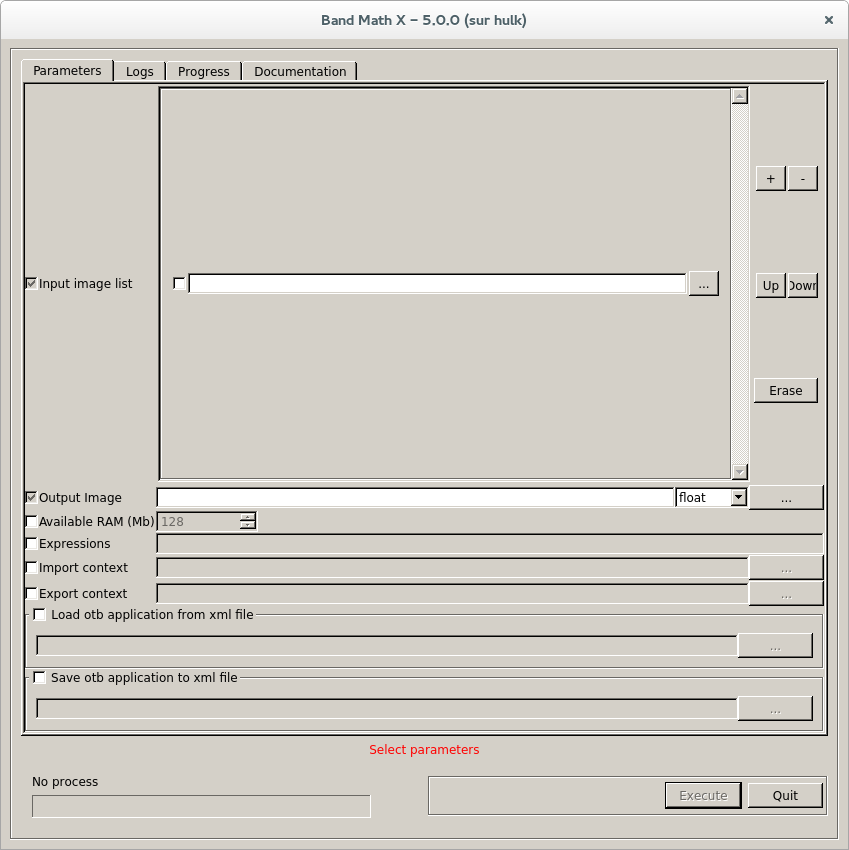
\includegraphics[width=7cm,height=7cm]{images/bandmathx.png}

\end{frame}


\end{frame}

\begin{frame}
\frametitle{Real life examples}

\begin{itemize}
\item Conversion 12 bits RGBNIR to 8 bits RGB with gamma correction : (im1 - min) div ( (max-min) pw gamma )
\item Many vegetation indices into a single image : im1b4/im1b1 ; (im1b4-im1b1) / (im1b4+im1b1) ; (alpha*im1b4-im1b1) / (alpha*im1b4+im1b1)
\item Single scale retinex : vlog(im1) - vlog( mean(im1b1N5x5,im1b2N5x5,im1b3N5x5,im1b4N5x5) )
\newline
\newline
\item Spectral angle : vacos( dotpr(im1,im2) div (vnorm(im1) mult vnorm(im2)) )
\item Maps of local maxima/minima : (im1b1 $>$ vmax(im1b1N5x5))?\{1\}:\{0\}
\end{itemize} 

\end{frame}


\end{document}
